% 41039 Programming 1 revision; shared style copied from the established Week 4 deck.
\documentclass[aspectratio=169]{beamer}
\makeatletter

\usepackage{lmodern}
\usepackage{booktabs}
\usepackage{array}
\usepackage{graphicx}
\usepackage{xcolor}
\usepackage{listings}
\usepackage{pifont}
\usepackage{enumitem}
\usepackage[most]{tcolorbox}
\usepackage{tikz}
\usetikzlibrary{shapes.geometric, arrows.meta, positioning}

% Beamer's default enumerate label expands to itself once enumitem takes the optional
% argument, and TeX runs out of input stack. An explicit label breaks the loop.
\setlist[enumerate]{label=\arabic*.}
\setlist[itemize]{label=\usebeamertemplate{itemize item}}

\definecolor{bkblue}{RGB}{0,70,140}
\definecolor{bktitlebg}{RGB}{64,116,169}
\definecolor{codebg}{RGB}{244,246,249}
\definecolor{codecmt}{RGB}{110,120,130}
\definecolor{codegray}{RGB}{110,120,135}
\definecolor{codestr}{RGB}{150,60,20}
\definecolor{badred}{RGB}{185,40,40}
\definecolor{goodgreen}{RGB}{20,125,70}
\definecolor{srcgrey}{RGB}{105,115,128}

\usetheme{default}
\useinnertheme{rounded}
\setbeamertemplate{navigation symbols}{}

\setbeamercolor{titlelike}{bg=bktitlebg,fg=white}
\setbeamercolor{frametitle}{fg=bkblue,bg=}
\setbeamercolor{author}{fg=bkblue}
\setbeamercolor{institute}{fg=bkblue}
\setbeamercolor{section in toc}{fg=bkblue}
\setbeamerfont{frametitle}{size=\Large,series=\mdseries}
\setbeamerfont{title}{size=\Large,series=\bfseries}
\setbeamerfont{subtitle}{size=\normalsize,series=\bfseries}

\setbeamertemplate{frametitle}{%
  \vspace*{0.35em}%
  \begin{minipage}[b]{0.84\textwidth}%
    \usebeamerfont{frametitle}\usebeamercolor[fg]{frametitle}\insertframetitle%
  \end{minipage}\hfill%
  \begin{minipage}[b]{0.10\textwidth}%
    \raggedleft
\includegraphics[height=0.75cm]{bk-logo.png}%
  \end{minipage}\\[0.1em]%
  {\color{bkblue}\rule{\textwidth}{0.7pt}}%
}

\setbeamercolor{footbar}{bg=bkblue,fg=white}
\setbeamertemplate{footline}{%
  \begin{beamercolorbox}[wd=\paperwidth,ht=2.1ex,dp=1.1ex,leftskip=.3cm,rightskip=.3cm]{footbar}%
    \tiny\insertshorttitle\hfill\insertframenumber{}/\inserttotalframenumber%
  \end{beamercolorbox}%
}

\newcommand{\keyline}[1]{\vfill\begin{center}\textcolor{bkblue}{\textbf{#1}}\end{center}\vspace*{0.2em}}
\newcommand{\hd}[1]{\textbf{#1}}
\newcommand{\code}[1]{\texttt{#1}}
\newcommand{\srcline}[1]{{\color{srcgrey}\scriptsize #1\par}}
\newcommand{\srclink}[2]{\href{#1}{\texttt{#2}}}
\newcommand{\badlabel}[1]{\textcolor{badred}{\ding{55}~\textbf{#1}}}
\newcommand{\goodlabel}[1]{\textcolor{goodgreen}{\ding{51}~\textbf{#1}}}
\newcommand{\neutrallabel}[1]{\textcolor{bkblue}{\textbf{#1}}}
\newcommand{\timing}[2]{\hfill{\small\textcolor{bkblue}{\textbf{#1 \textbullet{} #2}}}}
% a blank to be filled in, numbered so the word bank can be checked against it
\newcommand{\blank}[1]{\underline{\hspace{1.1em}\textbf{(#1)}\hspace{1.1em}}}
\newcommand{\yes}{\textcolor{goodgreen}{\ding{51}}}
\newcommand{\no}{\textcolor{badred}{\ding{55}}}

% --- Stack and heap pictures (Draw it) --------------------------------------
\tikzset{
  sframe/.style={draw=bkblue, thick, fill=codebg, rounded corners=2pt, inner sep=4pt,
    font=\scriptsize\ttfamily, align=left, anchor=north west},
  ftitle/.style={font=\scriptsize\sffamily\bfseries, text=bkblue, anchor=south west},
  cell/.style={draw=bkblue, fill=white, font=\scriptsize\ttfamily, minimum width=0.62cm,
    minimum height=0.5cm, inner sep=1pt},
  atitle/.style={font=\scriptsize\ttfamily, text=bkblue, anchor=south west, inner sep=1pt},
  ref/.style={-{Stealth[length=5pt]}, thick, draw=bkblue!85!black},
  hd/.style={font=\small\sffamily\bfseries, text=bkblue},
}

\hypersetup{colorlinks=true, urlcolor=bkblue, linkcolor=bkblue}

% --- Question box: what the room is being asked --------------------------
\newtcolorbox{discussionbox}[1]{
  title=\textbf{#1}, coltitle=bkblue, colback=white, colframe=bkblue,
  colbacktitle=bkblue!10, boxrule=1pt, arc=3pt,
  left=6pt, right=6pt, top=4pt, bottom=4pt
}
% --- Answer box: revealed after they have committed to an answer ---------
\newtcolorbox{contextbox}[1]{
  title=\textbf{#1}, coltitle=white, colback=bkblue!5, colframe=bkblue,
  colbacktitle=bkblue!80, boxrule=0.6pt, arc=3pt,
  left=6pt, right=6pt, top=4pt, bottom=4pt
}

\lstdefinestyle{code}{
  basicstyle=\ttfamily\scriptsize,
  keywordstyle=\color{bkblue}\bfseries,
  commentstyle=\color{codecmt}\itshape,
  stringstyle=\color{codestr},
  backgroundcolor=\color{codebg},
  frame=leftline, framerule=1.2pt, rulecolor=\color{bkblue},
  xleftmargin=1.1em, framexleftmargin=1.1em,
  framexrightmargin=0.4em, framextopmargin=3pt, framexbottommargin=3pt,
  showstringspaces=false, columns=fullflexible, keepspaces=true,
  breaklines=true, aboveskip=0.6em, belowskip=0.6em,
}
\lstdefinestyle{bad}{style=code, rulecolor=\color{badred}, backgroundcolor=\color{badred!4}}
\lstdefinestyle{good}{style=code, rulecolor=\color{goodgreen}, backgroundcolor=\color{goodgreen!5}}
\lstset{style=code}
% listings' Python predates 3.10; teach it the soft keywords and constants this deck uses
\lstdefinelanguage{Py}[]{Python}{morekeywords={match,case,elif,True,False}}

\setbeamertemplate{title page}{%
  \vspace*{0.5em}
  \begin{centering}
    \begin{beamercolorbox}[sep=8pt,center,rounded=true,shadow=false]{title}
      \usebeamerfont{title}\inserttitle\par
      \ifx\insertsubtitle\@empty\else
        \vskip0.4em{\usebeamerfont{subtitle}\insertsubtitle\par}
      \fi
    \end{beamercolorbox}
    \vskip1.0em
    
\includegraphics[height=1.7cm]{bk-logo.png}
    \vskip1.0em
    {\usebeamercolor[fg]{author}\usebeamerfont{author}\insertauthor\par}
    \vskip0.5em
    {\usebeamercolor[fg]{institute}\usebeamerfont{institute}\insertinstitute\par}
    \vskip0.6em
    {\usebeamerfont{date}\insertdate\par}
  \end{centering}
}




\title[41039 Programming 1 --- Revision of Week 11]{41039 Programming 1}
\subtitle{Revision of Week 11: Designing object-oriented programs}
\author{Dr. Xuan-Bach Le\\ \small\texttt{le.xuan.bach@hcmut.edu.vn}}
\institute{\small Faculty of Computer Science and Engineering, HCMUT}
\date{September Session 2026}
\AtBeginSection[]{\begin{frame}{Outline}\tableofcontents[currentsection]\end{frame}}
\begin{document}

\begin{frame}{}
\titlepage
\end{frame}

\begin{frame}{How the revision session works}
\begin{discussionbox}{A recap before the next lecture}\small Write an answer before the reveal. Explain the state change, rule or contract that makes it follow. These are practice questions, with no new assessment requirements.\end{discussionbox}
\begin{columns}[T,onlytextwidth]
\column{0.48\textwidth}
\raggedright
\neutrallabel{Part 1: on your own}\begin{itemize}\small\item 6 short questions\item About 90 seconds per question\item Java and Python; name the language first\end{itemize}
\column{0.48\textwidth}
\raggedright
\neutrallabel{Part 2: teams of 3 or 4}\begin{itemize}\small\item Draw the model\item Spot the errors\item Predict the output\item Write and test the code\end{itemize}
\end{columns}
\keyline{A result needs a reason. A repair needs a counterexample.}
\end{frame}

\section{On your own}

\begin{frame}[fragile]{1. Keep the calculation in the expert}
\srcline{Java 8 excerpt: main statements and supporting types; commit to an outcome before the reveal.}
\begin{columns}[T,onlytextwidth]
\column{0.62\textwidth}
\raggedright
\begin{lstlisting}[style=code,language=Java]
Order order=new Order();
order.add(new Line(300,2));
order.add(new Line(150,1));
System.out.println(order.total());
class Line {
    private final int cents,quantity;
    Line(int cents,int quantity) { this.cents=cents; this.quantity=quantity; }
    int subtotal() { return cents*quantity; }
}
class Order {
    private final java.util.List<Line> lines=new java.util.ArrayList<Line>();
    void add(Line line) { lines.add(line); }
    int total() { int sum=0; for(Line line:lines) sum+=line.subtotal(); return sum; }
}
\end{lstlisting}

\column{0.34\textwidth}
\raggedright
\begin{onlyenv}<1>\begin{discussionbox}{Your answer}\small Predict the total. Which object should compute one line subtotal, and which object should aggregate the order?\end{discussionbox}\end{onlyenv}
\begin{onlyenv}<2>\begin{contextbox}{Answer}
\begin{lstlisting}[style=code]
750
\end{lstlisting}
\scriptsize\raggedright Each line computes its own subtotal; Order sums 600 and 150.
\end{contextbox}\end{onlyenv}
\end{columns}

\end{frame}

\begin{frame}[fragile]{2. Separate calculation from presentation}
\srcline{Python 3; commit to an outcome before the reveal.}
\begin{columns}[T,onlytextwidth]
\column{0.62\textwidth}
\raggedright
\begin{lstlisting}[style=code,language=Py]
class Order:
    def __init__(self, amounts): self.amounts=list(amounts)
    def total(self): return sum(self.amounts)
def format_receipt(order):
    return f"Total: {order.total()} cents"
order=Order([600,150])
print(order.total())
print(format_receipt(order))
\end{lstlisting}

\column{0.34\textwidth}
\raggedright
\begin{onlyenv}<1>\begin{discussionbox}{Your answer}\small What is the complete output? Which line or rule decides it?\end{discussionbox}\end{onlyenv}
\begin{onlyenv}<2>\begin{contextbox}{Answer}
\begin{lstlisting}[style=code]
750
Total: 750 cents
\end{lstlisting}
\scriptsize\raggedright The calculation returns a number; the formatter builds a human-readable receipt from that result.
\end{contextbox}\end{onlyenv}
\end{columns}

\end{frame}

\begin{frame}[fragile]{3. An extensible pricing rule}
\srcline{Java 8 excerpt: main statements and supporting types; commit to an outcome before the reveal.}
\begin{columns}[T,onlytextwidth]
\column{0.62\textwidth}
\raggedright
\begin{lstlisting}[style=code,language=Java]
Basket basket=new Basket(new StudentPrice());
System.out.println(basket.price(1000));
interface PriceRule { int apply(int cents); }
class StudentPrice implements PriceRule {
    public int apply(int cents) { return cents*80/100; }
}
class Basket {
    private final PriceRule rule;
    Basket(PriceRule rule) { this.rule=rule; }
    int price(int cents) { return rule.apply(cents); }
}
\end{lstlisting}

\column{0.34\textwidth}
\raggedright
\begin{onlyenv}<1>\begin{discussionbox}{Your answer}\small What prints? Which parts depend on the pricing interface, and how does that help when adding a new policy?\end{discussionbox}\end{onlyenv}
\begin{onlyenv}<2>\begin{contextbox}{Answer}
\begin{lstlisting}[style=code]
800
\end{lstlisting}
\scriptsize\raggedright StudentPrice applies the 80\% policy. Basket depends on the PriceRule abstraction and receives its collaborator through the constructor. This supports dependency inversion and lets a new policy extend the behaviour without changing Basket.price.
\end{contextbox}\end{onlyenv}
\end{columns}

\end{frame}

\begin{frame}[fragile]{4. Inject a function in Python}
\srcline{Python 3; commit to an outcome before the reveal.}
\begin{columns}[T,onlytextwidth]
\column{0.62\textwidth}
\raggedright
\begin{lstlisting}[style=code,language=Py]
def student_price(cents): return cents*80//100
def regular_price(cents): return cents
class Basket:
    def __init__(self, rule): self.rule=rule
    def price(self, cents): return self.rule(cents)
print(Basket(student_price).price(1000))
print(Basket(regular_price).price(1000))
\end{lstlisting}

\column{0.34\textwidth}
\raggedright
\begin{onlyenv}<1>\begin{discussionbox}{Your answer}\small What is the complete output? Which line or rule decides it?\end{discussionbox}\end{onlyenv}
\begin{onlyenv}<2>\begin{contextbox}{Answer}
\begin{lstlisting}[style=code]
800
1000
\end{lstlisting}
\scriptsize\raggedright The caller supplies different policies to the same Basket implementation.
\end{contextbox}\end{onlyenv}
\end{columns}

\end{frame}

\begin{frame}[fragile]{5. Substitutability includes behaviour}
\srcline{Java 8; commit to an outcome before the reveal.}
\begin{columns}[T,onlytextwidth]
\column{0.62\textwidth}
\raggedright
\begin{lstlisting}[style=code,language=Java]
public class Demo {
    static void fill(java.util.List<Integer> xs) { xs.add(2); xs.add(3); }
    public static void main(String[] args) {
        java.util.List<Integer> a=new java.util.ArrayList<Integer>();
        java.util.List<Integer> b=new java.util.LinkedList<Integer>();
        fill(a); fill(b);
        System.out.println(a.equals(b));
        System.out.println(a.get(0));
    }
}
\end{lstlisting}

\column{0.34\textwidth}
\raggedright
\begin{onlyenv}<1>\begin{discussionbox}{Your answer}\small Predict the output. Would a replacement List remain substitutable if its add method inserted at the front?\end{discussionbox}\end{onlyenv}
\begin{onlyenv}<2>\begin{contextbox}{Answer}
\begin{lstlisting}[style=code]
true
2
\end{lstlisting}
\scriptsize\raggedright Both implementations preserve append order, so their contents are equal and begin with 2. A replacement that prepended instead would violate the List contract. Matching a method signature does not prove behavioural substitutability.
\end{contextbox}\end{onlyenv}
\end{columns}

\end{frame}

\begin{frame}[fragile]{6. A narrow capability}
\srcline{Python 3; commit to an outcome before the reveal.}
\begin{columns}[T,onlytextwidth]
\column{0.62\textwidth}
\raggedright
\begin{lstlisting}[style=code,language=Py]
class Screen:
    def send(self, message): return "screen: "+message
class Recorder:
    def __init__(self): self.messages=[]
    def send(self, message):
        self.messages.append(message)
        return "recorded"
def notify(channel, message): return channel.send(message)
recorder=Recorder()
print(notify(recorder,"Ready"))
print(recorder.messages)
\end{lstlisting}

\column{0.34\textwidth}
\raggedright
\begin{onlyenv}<1>\begin{discussionbox}{Your answer}\small What is the complete output? Which line or rule decides it?\end{discussionbox}\end{onlyenv}
\begin{onlyenv}<2>\begin{contextbox}{Answer}
\begin{lstlisting}[style=code]
recorded
['Ready']
\end{lstlisting}
\scriptsize\raggedright The recorder fulfils the same send capability and stores the message for inspection.
\end{contextbox}\end{onlyenv}
\end{columns}

\end{frame}

\section{Team round 1: draw the model}

\begin{frame}{Form teams}
\begin{itemize}[itemsep=0.8em]\item Teams of 3 or 4. One shared sheet, one spokesperson.\item For each challenge, record the result and the reason.\item Rotate the spokesperson. Other teams can challenge an explanation.\item The final task has starter files and a Java/Python solution pair.\end{itemize}\keyline{Discuss first. Commit to an answer. Then compare with the reveal.}
\end{frame}

\begin{frame}[fragile]{Draw it: A responsibility map for an order}
\begin{columns}[T,onlytextwidth]
\column{0.62\textwidth}
\raggedright
\begin{lstlisting}[style=code,language=Java]
Line a=new Line(300,2);
Line b=new Line(150,1);
Order order=new Order(a,b);
System.out.println(order.total());
class Line {
    private final int cents,quantity;
    Line(int cents,int quantity) { this.cents=cents; this.quantity=quantity; }
    int subtotal() { return cents*quantity; }
}
class Order {
    private final Line a,b;
    Order(Line a,Line b) { this.a=a; this.b=b; }
    int total() { return a.subtotal()+b.subtotal(); }
}
\end{lstlisting}

\column{0.34\textwidth}
\raggedright
\begin{discussionbox}{Four minutes}\small Draw the flow and responsibilities after the shown operations. Label the important state. Mark what is shared, what changes, or which path handles failure. Predict every output line.\end{discussionbox}
\end{columns}
\par\srcline{\href{../../weeks/week-11.html}{Course website: Week 11}. Complete programs accompany this deck.}

\end{frame}

\begin{frame}[fragile]{Draw it: one answer}
\begin{columns}[T,onlytextwidth]
\column{0.66\textwidth}
\raggedright
\resizebox{\linewidth}{!}{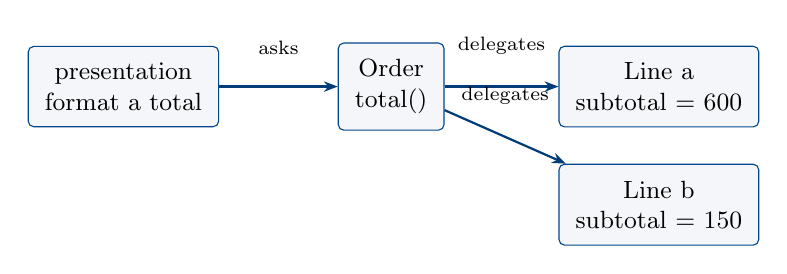
\begin{tikzpicture}
\node[draw=bkblue,rounded corners=2pt,fill=codebg,align=center,inner sep=6pt,font=\small] (ui) at (0,0) {presentation\\[0pt] format a total};
\node[draw=bkblue,rounded corners=2pt,fill=codebg,align=center,inner sep=6pt,font=\small] (order) at (3.4,0) {Order\\[0pt] total()};
\node[draw=bkblue,rounded corners=2pt,fill=codebg,align=center,inner sep=6pt,font=\small] (a) at (6.8,0) {Line a\\[0pt] subtotal = 600};
\node[draw=bkblue,rounded corners=2pt,fill=codebg,align=center,inner sep=6pt,font=\small] (b) at (6.8,-1.5) {Line b\\[0pt] subtotal = 150};
\draw[ref] (ui) -- node[above=8pt,font=\scriptsize]{asks} (order);
\draw[ref] (order) -- node[above=8pt,font=\scriptsize]{delegates} (a);
\draw[ref] (order) -- node[above=8pt,font=\scriptsize]{delegates} (b);
\end{tikzpicture}}

\column{0.3\textwidth}
\raggedright
\begin{contextbox}{Output}\begin{lstlisting}[style=code]
750
\end{lstlisting}
\end{contextbox}
\end{columns}
\vspace{0.8em}
\small Line is the information expert for its own subtotal. Order aggregates its lines. Presentation can change its wording without changing the arithmetic.
\par\srcline{\href{../../weeks/week-11.html}{Course website: Week 11}. Complete programs accompany this deck.}

\end{frame}

\section{Team round 2: spot the errors}

\begin{frame}[fragile]{Spot the errors 1: Java (5 min)}
\begin{discussionbox}{Contract}\small With HalfPrice, total(1000) returns 500 without printing. Main prints one line.\end{discussionbox}
\begin{columns}[T,onlytextwidth]
\column{0.48\textwidth}
\raggedright
\begin{lstlisting}[style=bad,language=Java,numbers=left,numberstyle=\tiny\color{codegray},firstnumber=1,numbersep=0.7em]
public class Broken {
    public static void main(String[] args) {
        Checkout c=new Checkout(new HalfPrice());
        System.out.println(c.total(1000));
    }
}
interface Pricing { int apply(int cents); }
class Regular implements Pricing {
    public int apply(int cents) { return cents; }
}
class HalfPrice implements Pricing {
\end{lstlisting}

\column{0.48\textwidth}
\raggedright
\begin{lstlisting}[style=bad,language=Java,numbers=left,numberstyle=\tiny\color{codegray},firstnumber=12,numbersep=0.7em]
    public int apply(int cents) { return cents/2; }
}
class Checkout {
    private final Pricing rule;
    Checkout(Pricing rule) { this.rule=new Regular(); }
    int total(int cents) {
        System.out.println("charging");
        return rule.apply(cents);
    }
}
\end{lstlisting}

\end{columns}

\end{frame}

\begin{frame}[fragile]{Spot the errors 1: answers}
\begin{columns}[T,onlytextwidth]
\column{0.58\textwidth}
\raggedright
\begin{contextbox}{The repairs}\footnotesize\begin{itemize}[itemsep=0.45em]\item \textbf{L16:} Keep the supplied Pricing collaborator instead of constructing an unrelated fixed policy.\item \textbf{L18:} A calculation-only total method should return the charge without choosing a presentation side effect.\end{itemize}\end{contextbox}
\column{0.38\textwidth}
\raggedright
\badlabel{Original program}\begin{lstlisting}[style=code]
charging
1000
\end{lstlisting}
\goodlabel{After the repairs}\begin{lstlisting}[style=code]
500
\end{lstlisting}

\end{columns}
\par\srcline{\href{../../weeks/week-11.html}{Course website: Week 11}. Complete programs accompany this deck.}

\end{frame}

\begin{frame}[fragile]{Spot the errors 2: Python (5 min)}
\begin{discussionbox}{Contract}\small Count and labels must agree at the boundary, and one function must own the pass rule.\end{discussionbox}
\begin{columns}[T,onlytextwidth]
\column{0.48\textwidth}
\raggedright
\begin{lstlisting}[style=bad,language=Py,numbers=left,numberstyle=\tiny\color{codegray},firstnumber=1,numbersep=0.7em]
def passes(mark): return mark>50

def count_passes(marks):
    return sum(passes(mark) for mark in marks)
def labels(marks):
\end{lstlisting}

\column{0.48\textwidth}
\raggedright
\begin{lstlisting}[style=bad,language=Py,numbers=left,numberstyle=\tiny\color{codegray},firstnumber=6,numbersep=0.7em]
    return ["P" if mark>=50 else "F" for mark in marks]

marks=[49,50,85]
print(count_passes(marks))
print(labels(marks))
\end{lstlisting}

\end{columns}

\end{frame}

\begin{frame}[fragile]{Spot the errors 2: answers}
\begin{columns}[T,onlytextwidth]
\column{0.58\textwidth}
\raggedright
\begin{contextbox}{The repairs}\footnotesize\begin{itemize}[itemsep=0.45em]\item \textbf{L1:} Include the exact pass boundary: 50 passes.\item \textbf{L6:} Use passes(mark) here too, so counting and labels share one source of the pass rule.\end{itemize}\end{contextbox}
\column{0.38\textwidth}
\raggedright
\badlabel{Original program}\begin{lstlisting}[style=code]
1
['F', 'P', 'P']
\end{lstlisting}
\goodlabel{After the repairs}\begin{lstlisting}[style=code]
2
['F', 'P', 'P']
\end{lstlisting}

\end{columns}
\par\srcline{\href{../../weeks/week-11.html}{Course website: Week 11}. Complete programs accompany this deck.}

\end{frame}

\section{Team round 3: predict the output}

\begin{frame}[fragile]{Predict 1: A policy and a common caller}
\begin{columns}[T,onlytextwidth]
\column{0.62\textwidth}
\raggedright
\begin{lstlisting}[style=code,language=Java]
public class Demo {
    static int charge(Price rule,int cents) { return rule.apply(cents); }
    public static void main(String[] args) {
        Price[] rules={new Regular(),new Half()};
        for(Price rule:rules) System.out.println(charge(rule,101));
    }
}
interface Price { int apply(int cents); }
class Regular implements Price {
    public int apply(int cents) { return cents; }
}
class Half implements Price {
    public int apply(int cents) { return cents/2; }
}
\end{lstlisting}

\column{0.34\textwidth}
\raggedright
\begin{discussionbox}{Three minutes}\small Write every line in order. Explain the first state change, alias, dispatch decision or exception that controls the result. Then propose one change that alters the output.\end{discussionbox}
\end{columns}
\par\srcline{\href{../../weeks/week-11.html}{Course website: Week 11}. Complete programs accompany this deck.}

\end{frame}

\begin{frame}[fragile]{Predict 1: answer}
\begin{columns}[T,onlytextwidth]
\column{0.42\textwidth}
\raggedright
\begin{lstlisting}[style=code]
101
50
\end{lstlisting}

\column{0.54\textwidth}
\raggedright
\begin{contextbox}{Why}\small charge depends only on Price. The two objects select different policies; integer division truncates the fractional cent for Half.\end{contextbox}
\end{columns}
\par\srcline{\href{../../weeks/week-11.html}{Course website: Week 11}. Complete programs accompany this deck.}

\end{frame}

\begin{frame}[fragile]{Predict 2: One capability, observable interactions}
\begin{columns}[T,onlytextwidth]
\column{0.62\textwidth}
\raggedright
\begin{lstlisting}[style=code,language=Py]
class Recorder:
    def __init__(self): self.messages=[]
    def send(self,text):
        self.messages.append(text)
        return len(self.messages)
def notify(channel,text): return channel.send(text)
a=Recorder()
b=a
print(notify(b,"Ready"))
print(notify(a,"Go"))
print(a.messages,b.messages is a.messages)
\end{lstlisting}

\column{0.34\textwidth}
\raggedright
\begin{discussionbox}{Three minutes}\small Write every line in order. Explain the first state change, alias, dispatch decision or exception that controls the result. Then propose one change that alters the output.\end{discussionbox}
\end{columns}
\par\srcline{\href{../../weeks/week-11.html}{Course website: Week 11}. Complete programs accompany this deck.}

\end{frame}

\begin{frame}[fragile]{Predict 2: answer}
\begin{columns}[T,onlytextwidth]
\column{0.42\textwidth}
\raggedright
\begin{lstlisting}[style=code]
1
2
['Ready', 'Go'] True
\end{lstlisting}

\column{0.54\textwidth}
\raggedright
\begin{contextbox}{Why}\small The recorder is a test collaborator. Both variables identify one recorder, so both requests add to the same history.\end{contextbox}
\end{columns}
\par\srcline{\href{../../weeks/week-11.html}{Course website: Week 11}. Complete programs accompany this deck.}

\end{frame}

\section{Team round 4: write the code}

\begin{frame}[fragile]{Code it: specification}
\begin{discussionbox}{Information experts in an order}\small Read n, then n pairs: non-negative unit price in cents and quantity. Line.subtotal computes the product. Order.total sums the line subtotals. Print the total. Explain which responsibility belongs to each class.\end{discussionbox}
\begin{columns}[T,onlytextwidth]
\column{0.48\textwidth}
\raggedright
\neutrallabel{Example input}\begin{lstlisting}[style=code]
2
300 2
150 1
\end{lstlisting}

\column{0.48\textwidth}
\raggedright
\neutrallabel{Expected output}\begin{lstlisting}[style=code]
750
\end{lstlisting}

\end{columns}
\small Eight minutes. One Java team and one Python team at the keyboard. Other teams produce a boundary test and explain which wrong implementation it would expose.
\end{frame}

\begin{frame}[fragile]{Code it: Java solution}
\begin{lstlisting}[style=code,language=Java,numbers=left,numberstyle=\tiny\color{codegray},firstnumber=1,numbersep=0.7em]
import java.util.*;
Scanner sc=new Scanner(System.in);
int n=sc.nextInt();
Order order=new Order();
for(int i=0;i<n;i++) order.add(new Line(sc.nextInt(),sc.nextInt()));
System.out.println(order.total());
class Line {
    private final int price,quantity;
    Line(int price,int quantity) { this.price=price; this.quantity=quantity; }
    int subtotal() { return price*quantity; }
}
class Order {
    private final List<Line> lines=new ArrayList<Line>();
    void add(Line line) { lines.add(line); }
    int total() { int total=0; for(Line line:lines) total+=line.subtotal(); return total; }
}
\end{lstlisting}
\par\srcline{\href{../../weeks/week-11.html}{Course website: Week 11}. Complete programs accompany this deck.}

\end{frame}

\begin{frame}[fragile]{Code it: Python solution}
\begin{lstlisting}[style=code,language=Py,numbers=left,numberstyle=\tiny\color{codegray},firstnumber=1,numbersep=0.7em]
class Line:
    def __init__(self,price,quantity): self.price,self.quantity=price,quantity
    def subtotal(self): return self.price*self.quantity
class Order:
    def __init__(self): self.lines=[]
    def add(self,line): self.lines.append(line)
    def total(self): return sum(line.subtotal() for line in self.lines)
order=Order()
n=int(input())
for _ in range(n):
    price,quantity=map(int,input().split())
    order.add(Line(price,quantity))
print(order.total())
\end{lstlisting}
\par\srcline{\href{../../weeks/week-11.html}{Course website: Week 11}. Complete programs accompany this deck.}

\end{frame}

\begin{frame}{Code it: the tests}
\footnotesize {\scriptsize A slash separates input lines; (blank) denotes an empty line.\par}\medskip \textbf{Test 1}\par \code{2 / 300 2 / 150 1}\par \textbf{Output:} \code{750}\par\medskip \textbf{Test 2}\par \code{0}\par \textbf{Output:} \code{0}\par\medskip \textbf{Test 3}\par \code{3 / 0 10 / 100 0 / 1 1}\par \textbf{Output:} \code{1}\par\medskip \keyline{Explain why each test is present, not only whether it passes.}
\end{frame}

\section{Wrapping up}

\begin{frame}{What you should now be able to explain}
\begin{itemize}[itemsep=0.6em]\item Assign behaviour to the object with the needed information.\item Keep computation independent of display and file choices.\item Supply collaborators through a useful abstraction.\item Use SOLID, GRASP, DRY and YAGNI to justify concrete decisions.\end{itemize}\vfill\small Return to the matching week page for runnable examples and further practice. Bring one unresolved prediction or counterexample to the next class.\par\srcline{\href{../../weeks/week-11.html}{Course website: Week 11}. Complete programs accompany this deck.}

\end{frame}

\end{document}
